\section{Introduction}
	The significant improvement of machine learning (ML) over the decades has led to a host of applications of ML in  high-stake decision-making such as college admission~\cite{martinez2021using}, hiring of employees~\cite{ajunwa2016hiring}, and recidivism prediction~\cite{tollenaar2013method,dressel2018accuracy}. ML algorithms often have an accuracy-centric learning objective, which may cause them to be biased towards certain part of the dataset belonging to a certain economically or socially sensitive groups~\cite{landy1978correlates,zliobaite2015relation,berk2019accuracy}.
%	Fairness in Machine Learning (ML) has gained a significant focus  in recent years as ML algorithms are deployed in high-stake decision-making, such as college admission, hiring of employees, and recidivism prediction. Thus, if the ML algorithm is biased towards certain part of the dataset belonging to certain economically or socially sensitive groups, it can cause adverse effects in real-life.
	 The following example illustrates a plausible case of unfairness induced by ML algorithms. 
	\begin{example}\label{fvgm_example:intro}
		Following~\cite[Example 1.]{ghosh2020justicia}, let us consider an ML problem where the classifier decides the eligibility of an individual for health insurance given their income and fitness (Figure~\ref{fvgm_fig:example1}). Here, the sensitive feature `age' ($ A $) follows a Bernoulli distribution, and income ($ I $) and fitness ($ F $) follow Gaussian distributions. We generate 1000 samples from these distributions and use them to train a Support Vector Machine (SVM) classifier. The decision boundary of this classifier is $9.37I + 9.75F - 0.34A \ge 9.4$, where $A = 1$ denotes the sensitive group `age $ \ge $ 40'. This classifier selects an individual above and below $40$ years of age with probabilities $0.24$ and $0.86$, respectively. This illustrates a disparate treatment of individuals of two age groups by the SVM classifier. 
	\end{example}
%	The above example illustrates that even in simple scenarios, ML-based solutions can lead to disparate treatment. Motivated by studies indicating that such scenarios are rather not uncommon, there is a thrust in the research on the improvement of fairness in ML by proposing different notions of fairness definitions and fairness algorithms~\cite{hardt2016equality,kusner2017counterfactual,mehrabi2019survey}. 

%KSM: Make the two plots side by side
\begin{figure}[h!]
	%		{r}{0.25\textwidth}%\vspace*{-2.4em}
	\begin{center}
		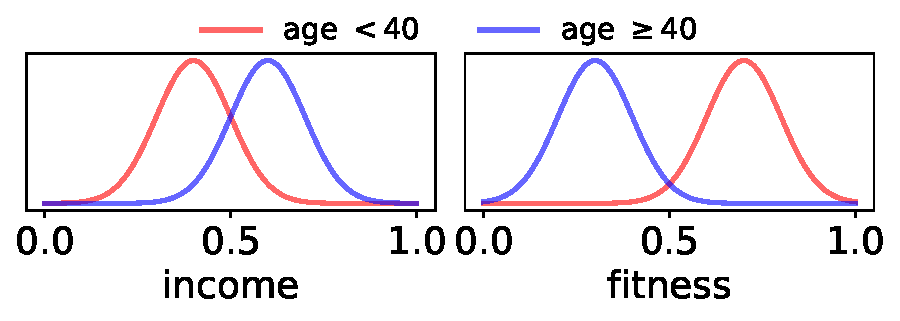
\includegraphics[scale = 0.4]{figures/fairness/fvgm/sanity_probability}
	\end{center}
%	\vspace*{-1em}
	\caption{Age-dependent distributions of income and fitness in Example~\ref{fvgm_example:intro}.}\label{fvgm_fig:example1}%\vspace*{-1.6em}
\end{figure}


	In order to identify and mitigate the bias of ML classifiers, different fairness definitions and fairness algorithms have been proposed~\cite{hardt2016equality,kusner2017counterfactual,mehrabi2019survey}.	In this paper, we focus on two families of fairness definitions: \textit{group} and \textit{causal} fairness. Group fairness metrics, such as disparate impact and equalized odds constrain the probability of the positive prediction of the classifier to be (almost) equal among different sensitive groups~\cite{dwork2012fairness,feldman2015certifying}.	On the other hand, causal fairness metrics assess the difference in positive predictions  if every feature in the causal relation  remains identical except the sensitive feature~\cite{nabi2018fair,zhang2018fairness}. The early works on \textit{fairness verification} focused on measuring fairness metrics of a classifier for a given dataset~\cite{aif360-oct-2018}. Naturally, such techniques were limited in enhancing confidence of users for wide deployment. Consequently, recent verifiers seek to achieve verification beyond  finite dataset and in turn focus on the  probability distribution of features~\cite{albarghouthi2017fairsquare, bastani2019probabilistic, ghosh2020justicia}.  More specifically, the input to the verifier is a classifier and  the probability distribution of features, and the output is an estimate of fairness metrics that the classifier obtains given the distribution. For Example~\ref{fvgm_example:intro}, a fairness verifier takes the SVM classifier and the distribution of features $ I, F, A $ as an input and outputs the probability of positive prediction of the classifier for  different sensitive groups. 
	
%	\red{Despite extensive efforts over the past few years, the scalability and accuracy of fairness verifiers remains a major challenge. In particular, the existing techniques fail to scale beyond {\em toy} examples. In this work, we seek to remedy the situation. As a first step, we focus on  \textit{linear classifiers}, which has attracted a significant attention from researchers in the context of fair algorithms~\cite{pleiss2017fairness,zafar2017fairness,dressel2018accuracy, john2020verifying}. At this point, it is worth highlighting that our empirical evaluation demonstrates that the existing techniques fail to scale beyond small examples or provide highly inaccurate estimates for comparatively {\em small} linear classifiers. }
 	
	
	In order to solve the fairness-verification problem, existing works have proposed two principled approaches.	Firstly, \cite{ghosh2020justicia} and \cite{albarghouthi2017fairsquare} propose formal methods that reduce the problem into a solution of an SSAT or an SMT~ formula respectively.	Secondly, \cite{bastani2019probabilistic} propose a sampling approach that relies on extensively enumerating the conditional probabilities of prediction given different sensitive features and thus, incurs high computational cost. Additionally, existing works assume feature independence of non-sensitive features and consider correlated features within a limited scope, such as conditional probabilities of non-sensitive features w.r.t. sensitive features and ignore correlations among non-sensitive features. As a result, the \textit{scalability} and \textit{accuracy} of existing  verifiers remains a major challenge.
	
	In this work, we seek to remedy the aforementioned situation. As a first step, we focus on  \textit{linear classifiers}, which has attracted significant attention from researchers in the context of fair algorithms~\cite{pleiss2017fairness,zafar2017fairness,dressel2018accuracy, john2020verifying}. At this point, it is worth highlighting that our empirical evaluation demonstrates that the existing techniques fail to scale beyond small examples or provide highly inaccurate estimates for comparatively {\em small} linear classifiers. 
	
%	In this paper, we argue that the above solution is not practical in verifying linear classifiers for two reasons: (i) the encoding of a linear classifier into an SSAT or an SMT formula or using a sampling approach suffer from scalability and (ii) ignoring correlations among all features results in an inaccurate estimate of fairness metrics. 	
	
	
%	Given multiple fairness definitions, fairness algorithms either \textit{preprocess} the training data~\cite{calmon2017optimized,kamiran2012data,zemel2013learning}, \textit{in-process} the classifier during training~\cite{zhang2018mitigating}, or \textit{post-process} the prediction of the trained classifiers~\cite{hardt2016equality,kamiran2012decision} to improve fairness. In contrast, fairness-attack algorithms try to manipulate the data or the classifier to worsen its fairness~\cite{solans2020poisoning}. 
	

	
%	\red{Among different ML classifiers, researcher This observation motivates us in asking the following research question: \textit{Can we design an efficient fairness verification framework for linear classifiers that can verify different fairness definitions and algorithms accurately?} 

	
	
%	
%	Considering the surge of research in ML fairness based on linear classifiers, we focus on designing a fairness verifier particularly tailored for linear classifiers. We further show novel applications of the verifier in practical fairness tasks, such as detecting fairness attacks and computing the source of unfairness in the level of input features.
%	
	

	
	
	\textbf{Our Contributions.} In this paper, we propose a fairness verification framework, namely {\fvgm} (\textbf{F}airness \textbf{V}erification with \textbf{G}raphical \textbf{M}odels), for accurately and efficiently verifying linear classifiers. {\fvgm} proposes a novel \textit{stochastic subset-sum} encoding for linear classifiers with an efficient pseudo-polynomial solution using dynamic programming. To address feature-correlations, {\fvgm} considers a graphical model, particularly a Bayesian Network that represents conditional dependence (and independence) among features in the form of a Directed Acyclic Graph (DAG).  
	%Finally, {\fvgm} encodes the Bayesian Network in a SSAT-based formulation to verify classifiers in CNF and in the stochastic subset-sum based formulation to verify linear classifiers.  
	Experimentally,  {\fvgm} is more accurate and scalable than existing fairness verifiers; {\fvgm} can verify group and causal fairness metrics for multiple fairness algorithms. We also demonstrate two novel applications of {\fvgm} as a fairness verifier: (a) detecting fairness attacks, and (b) computing Fairness Influence Functions (FIF) of features as a mean of identifying (un)fairness contribution of a subset of features. 
	


